\documentclass[12pt]{article}
\usepackage[a4paper,margin=1in]{geometry}
\usepackage{booktabs}
\usepackage{amsmath}
\usepackage{amssymb}
\usepackage{siunitx}
\usepackage{graphicx}
\usepackage{hyperref}
\usepackage{float}
\usepackage[font=footnotesize,labelfont=bf]{caption}
\usepackage{enumitem}
\usepackage{titlesec}
\usepackage{array}
\usepackage{multirow}

\setlength{\parskip}{4pt}
\setlength{\parindent}{0pt}
\setlength{\textfloatsep}{8pt plus 2pt minus 2pt}
\setlength{\floatsep}{6pt plus 2pt minus 2pt}
\setlength{\intextsep}{8pt plus 2pt minus 2pt}
\renewcommand{\topfraction}{0.9}
\renewcommand{\bottomfraction}{0.8}
\renewcommand{\textfraction}{0.07}
\renewcommand{\floatpagefraction}{0.8}
\titlespacing*{\section}{0pt}{10pt}{5pt}
\titlespacing*{\subsection}{0pt}{7pt}{3pt}

\title{COMP0047 --- Calibration Study:\\
Assessing and Improving Probabilistic Predictions of Market Regimes}
\author{\\
\small Individual Task --- April 2026}
\date{}

\begin{document}
\maketitle

% =====================================================================
\section{Introduction}
% =====================================================================

A well-calibrated probabilistic classifier is one whose predicted confidence levels
agree with observed frequencies: a model outputting $P(\text{bull}) = 0.85$ should
be correct approximately 85\% of the time within that confidence band.
Calibration is distinct from discrimination (measured by AUC); a model may rank
instances perfectly yet remain poorly calibrated.
In financial decision-making this distinction matters acutely.
An overconfident bear signal at a 20-day horizon can trigger premature portfolio
de-risking, incurring unnecessary transaction costs and opportunity losses.

This study investigates calibration quality for two classifier families, 
Logistic Regression (LR) and XGBoost (XGB), trained to predict bull/bear
equity-market regimes across three prediction horizons: 1 day, 5 days, and 20 days.
Two post-hoc calibration methods, Platt Scaling and Isotonic Regression, are applied
and evaluated.
The analysis is structured around three pre-registered hypotheses:

\begin{itemize}[leftmargin=1.5em,itemsep=2pt,topsep=4pt]
  \item[\textbf{H1}] XGBoost produces \emph{less} calibrated probability estimates than
    Logistic Regression across all three prediction horizons, as measured by
    Expected Calibration Error (ECE).
  \item[\textbf{H2}] Calibration error increases \emph{monotonically} with prediction
    horizon ($1\text{d} < 5\text{d} < 20\text{d}$) for both model families.
  \item[\textbf{H3}] Post-calibration, the ECE \emph{reduction} is greater for XGBoost
    than for Logistic Regression, since XGBoost has more systematic overconfidence
    to correct.
\end{itemize}

% =====================================================================
\section{Data}
% =====================================================================

\subsection{Dataset Description}

The dataset \texttt{labeled\_dataset.csv} is produced by the upstream group coursework regime-segmentation
pipeline (\texttt{notebooks/03\_regime\_segmentation}).
It consists of 8,066 daily observations of the S\&P 500 spanning January 1994 to
February 2026 collected from Yahoo Finance and macroeconomic data filled forward from the FRED database, each labelled as either \textit{bull} or \textit{bear}
according to a rule-based segmentation scheme.
Table~\ref{tab:dataset-summary} summarises the key properties.

\begin{table}[H]
\centering
\caption{Dataset overview.}
\label{tab:dataset-summary}
\begin{tabular}{ll}
\toprule
Property & Value \\
\midrule
Total observations & 8,066 \\
Date range & 1994-01-27 --- 2026-02-13 \\
Bull observations & 5,061 (62.8\%) \\
Bear observations & 3,005 (37.2\%) \\
Total features & 25 \\
\bottomrule
\end{tabular}
\end{table}

\subsection{Features}

Twenty-five features spanning price dynamics, technical indicators, and
macroeconomic variables are used.
These are listed in Table~\ref{tab:features}.

\begin{table}[H]
\centering
\caption{Feature set used across all prediction horizons.}
\label{tab:features}
\small
\begin{tabular}{ll}
\toprule
Category & Features \\
\midrule
Price / Volume & \texttt{GSPC}, \texttt{SPY Volume} \\
Volatility & \texttt{VIX}, \texttt{VIX\_Change}, \texttt{VIX\_Change\_5d} \\
Returns & \texttt{Return}, \texttt{Return\_5d}, \texttt{Return\_20d}, \texttt{Return\_Smooth} \\
Technical indicators & \texttt{RSI\_14}, \texttt{MACD\_Line}, \texttt{MACD\_Signal}, \texttt{MACD\_Hist} \\
Macro variables & \texttt{GDP}, \texttt{Core\_Inflation}, \texttt{Unemployment}, \texttt{M2} \\
Macro YoY changes & \texttt{GDP\_YoY}, \texttt{Core\_Inflation\_YoY}, \texttt{M2\_YoY} \\
Calendar & \texttt{year}, \texttt{month}, \texttt{quarter} \\
Drawdown & \texttt{Peak}, \texttt{Drawdown} \\
\bottomrule
\end{tabular}
\end{table}

\subsection{Class Balance}

The dataset is moderately imbalanced: 62.8\% bull and 37.2\% bear.
This imbalance is preserved in both the training and test sets under the
chronological split (Section~\ref{sec:split}), ensuring that class proportions
are not artificially equalised, doing so would distort the calibration
diagnostic, because ECE is defined with respect to the true marginal outcome
frequency.

\subsection{Train / Test Split}
\label{sec:split}

Time-series data must not be shuffled before splitting, as random
shuffling would leak future information into the training set.
An 80/20 \emph{chronological} split is applied:

\begin{itemize}[leftmargin=1.5em,itemsep=2pt,topsep=4pt]
  \item \textbf{Training set}: 1994-01-27 to 2019-08-20 (6,436 observations).
  \item \textbf{Test set}: 2019-08-21 to 2026-01-15 (1,610 observations).
\end{itemize}

The test set bull/bear proportions per horizon are given in
Table~\ref{tab:test-balance}.

\begin{table}[H]
\centering
\caption{Test-set class distribution per prediction horizon.}
\label{tab:test-balance}
\begin{tabular}{lcc}
\toprule
Horizon & Bull (\%) & Bear (\%) \\
\midrule
1 day  & 73.7 & 26.3 \\
5 days & 74.0 & 26.0 \\
20 days & 74.9 & 25.1 \\
\bottomrule
\end{tabular}
\end{table}

Note that the test set (2019--2026) is more bullish than the full dataset (62.8\%),
as the post-2019 sample includes the extended post-COVID recovery rally.

% =====================================================================
\section{Target Construction}
% =====================================================================

Three forward-shifted binary targets are constructed, one per prediction horizon.
Let $r_t^{(h)}$ denote the regime label $h$ days into the future:
\begin{equation}
  y_t^{(h)} = \text{regime}_{t+h}, \quad h \in \{1, 5, 20\},
\end{equation}
where $y_t^{(h)} = 1$ (bull) and $y_t^{(h)} = 0$ (bear).

The target is shifted \emph{forward} relative to today's features (rather than
shifting features backward), which correctly simulates predicting future regime
state from present-day observable information.
After dropping the trailing $h$ observations required for target construction
(due to the forward shift), the working dataset contains 8,046 rows.

The choice to predict regime labels rather than point returns reflects the
intended downstream use case: regime-conditioned portfolio allocation, where a
coarse bull/bear signal is sufficient to tilt exposures.
Predicting the multi-day forward label also means the target aggregates
information over $h$ steps, so harder calibration at longer horizons is expected.

% =====================================================================
\section{Methodology}
% =====================================================================

\subsection{Baseline Models}

Two classifier families are evaluated:

\paragraph{Logistic Regression (LR).}
Logistic Regression models the log-odds of the bull class as a linear function
of the input features:
\begin{equation}
  \log \frac{P(y=1 \mid \mathbf{x})}{P(y=0 \mid \mathbf{x})} = \mathbf{w}^\top \mathbf{x} + b,
\end{equation}
so that predicted probabilities are produced via the sigmoid function.
Because the output probability is \emph{derived} from the sigmoid of a linear
combination, LR is often considered \textit{inherently} better calibrated than
non-parametric ensemble methods.
We use \texttt{sklearn.linear\_model.LogisticRegression} with \texttt{max\_iter=2000}
(to ensure convergence on the 25-dimensional input) and \texttt{random\_state=42}.

\paragraph{XGBoost (XGB).}
Gradient-boosted trees learn additive combinations of shallow decision trees
(here: \texttt{max\_depth=4}, \texttt{n\_estimators=200},
\texttt{learning\_rate=0.05}).
Unlike LR, XGBoost produces probabilities by applying a sigmoid to the raw
boosted score, but the tree ensemble optimises a log-loss objective without
any architectural guarantee of calibration.
Empirically, tree-based models tend to produce \emph{overconfident} predictions
because they push scores toward the extremes of the probability simplex,
particularly when the ensemble is deep or well-regularised
(Niculescu-Mizil \& Caruana, 2005).
This motivates H1.

Both models are trained independently for each of the three horizons, yielding
six uncalibrated probability vectors for evaluation.

\subsection{Calibration Metrics}

\paragraph{Expected Calibration Error (ECE).}
ECE partitions predictions into $B = 10$ equal-width bins over $[0, 1]$ and
computes the weighted mean absolute deviation between bin-level accuracy and
mean confidence:
\begin{equation}
  \text{ECE} = \sum_{b=1}^{B} \frac{|\mathcal{B}_b|}{n}
    \left|\,\text{acc}(\mathcal{B}_b) - \text{conf}(\mathcal{B}_b)\,\right|,
  \label{eq:ece}
\end{equation}
where $|\mathcal{B}_b|$ is the number of samples in bin $b$,
$\text{acc}(\mathcal{B}_b) = \frac{1}{|\mathcal{B}_b|}\sum_{i\in\mathcal{B}_b}y_i$,
and $\text{conf}(\mathcal{B}_b) = \frac{1}{|\mathcal{B}_b|}\sum_{i\in\mathcal{B}_b}\hat{p}_i$.
A perfectly calibrated model has $\text{ECE} = 0$.
ECE is chosen as the primary metric because (i) it provides an interpretable
``average miscalibration in probability units'' and (ii) it is the standard
benchmark in the calibration literature (Guo et al., 2017).

\paragraph{Maximum Calibration Error (MCE).}
MCE reports the \emph{worst-case} bin deviation:
\begin{equation}
  \text{MCE} = \max_{b=1}^{B}
    \left|\,\text{acc}(\mathcal{B}_b) - \text{conf}(\mathcal{B}_b)\,\right|.
  \label{eq:mce}
\end{equation}
MCE is a more conservative metric and is reported alongside ECE to capture
tail miscalibration.

\paragraph{Supporting metrics.}
The Brier Score,
$\text{BS} = \frac{1}{n}\sum_i (\hat{p}_i - y_i)^2$,
measures probabilistic accuracy in a proper scoring rule sense.
Log-loss (cross-entropy) and AUC are reported for completeness; note that
AUC is calibration-invariant, a model can achieve high AUC while remaining
poorly calibrated.

\subsection{Post-Hoc Calibration Methods}
\label{sec:calib-methods}

Post-hoc calibration refers to fitting a \emph{secondary} correction function
$g: [0,1] \to [0,1]$ that maps raw model scores $\hat{p}$ to calibrated
probabilities $\tilde{p} = g(\hat{p})$, without retraining the underlying
classifier.
Two methods are compared:

\paragraph{Platt Scaling (sigmoid calibration).}
Platt (1999) proposed fitting a logistic regression on top of the raw scores:
\begin{equation}
  \tilde{p} = \sigma(a \cdot f(\mathbf{x}) + b)
    = \frac{1}{1 + \exp(-(a f(\mathbf{x}) + b))},
\end{equation}
where $a$ and $b$ are scalar parameters fitted by maximum likelihood on
held-out data.
Platt Scaling is \emph{parametric}, it assumes the miscalibration is
monotone and well-approximated by a sigmoid warp.
This makes it fast, statistically efficient on small calibration sets, and
robust to overfitting.
The disadvantage is that it cannot correct non-monotone patterns (e.g., an
S-shaped reliability curve).

\paragraph{Isotonic Regression.}
Isotonic Regression (Zadrozny \& Elkan, 2002) fits a piecewise-constant
monotone non-decreasing function to the raw scores by solving:
\begin{equation}
  \min_{\tilde{p}\,:\,\text{isotonic}} \sum_i (\tilde{p}_i - y_i)^2.
\end{equation}
It is \emph{non-parametric}, it imposes only monotonicity, not a
functional form.
This flexibility enables it to correct arbitrary monotone miscalibration,
but at the cost of higher variance on small calibration sets (risk of overfitting).

\paragraph{Cross-validated calibration.}
Both calibrators are fitted using \\ \texttt{CalibratedClassifierCV(cv=5)},
which trains the calibration layer on 5-fold cross-validated out-of-fold
predictions from the training set.
This prevents the calibrator from seeing its own training data, avoiding
optimistic bias in the calibration fit.
The calibrated model is then evaluated on the held-out test set.

The choice to compare Platt Scaling with Isotonic Regression is motivated by
the need to span the parametric--non-parametric axis.
If XGBoost's miscalibration is predominantly monotone (as expected from
overconfident sigmoid outputs), both methods should help; if the reliability
curve is irregular, Isotonic Regression should outperform Platt Scaling.

% =====================================================================
\section{Results: Baseline (Pre-Calibration)}
% =====================================================================

\subsection{Discriminative Performance}

Table~\ref{tab:baseline-auc} reports AUC for all six baseline models.
Both classifiers achieve strong discrimination at 1 day (AUC $> 0.88$),
moderate discrimination at 5 days, and only marginally above chance at
20 days.
The 20-day horizon is substantially harder because the regime label becomes
increasingly uncorrelated with today's features as the forecast window grows.

\begin{table}[H]
\centering
\caption{Baseline AUC on the test set. Values rounded to 3 significant digits.}
\label{tab:baseline-auc}
\begin{tabular}{lcc}
\toprule
Horizon & LR AUC & XGB AUC \\
\midrule
1 day  & 0.901 & 0.881 \\
5 days & 0.853 & 0.868 \\
20 days & 0.641 & 0.594 \\
\bottomrule
\end{tabular}
\end{table}

A key observation is that LR outperforms XGB at 1 day and 20 days, while
XGB is slightly better at 5 days.
This reversal at 5 days suggests that the intermediate horizon benefits from
the non-linear interactions captured by boosted trees.

\subsection{Calibration Metrics Before Calibration}

Table~\ref{tab:pre-calib} presents the full set of pre-calibration metrics.
All five metrics (ECE, MCE, Brier Score, Log-Loss, AUC) are shown for
each model--horizon combination.

\begin{table}[H]
\centering
\caption{Pre-calibration metrics on the test set. ECE and MCE computed with
$B=10$ bins. Values rounded to 3 significant digits.}
\label{tab:pre-calib}
\begin{tabular}{llccccc}
\toprule
Horizon & Model & ECE & MCE & Brier & Log-Loss & AUC \\
\midrule
\multirow{2}{*}{1 day}
  & Logistic  & 0.151 & 0.469 & 0.167 & 0.656 & 0.901 \\
  & XGBoost   & 0.163 & 0.456 & 0.163 & 0.591 & 0.881 \\
\midrule
\multirow{2}{*}{5 days}
  & Logistic  & 0.199 & 0.532 & 0.208 & 0.792 & 0.853 \\
  & XGBoost   & 0.190 & 0.391 & 0.180 & 0.614 & 0.868 \\
\midrule
\multirow{2}{*}{20 days}
  & Logistic  & 0.357 & 0.621 & 0.351 & 1.176 & 0.641 \\
  & XGBoost   & 0.370 & 0.695 & 0.354 & 1.013 & 0.594 \\
\bottomrule
\end{tabular}
\end{table}

\subsection{Reliability Diagrams (Pre-Calibration)}

Figure~\ref{fig:reliability-pre} shows the reliability diagrams for both
models across all three horizons.
Points \emph{above} the diagonal indicate underconfidence (the model assigns
lower confidence than the true frequency warrants); points \emph{below}
indicate overconfidence.
The shaded area visualises the signed gap between the calibration curve and
perfect calibration.

\begin{figure}[H]
\centering
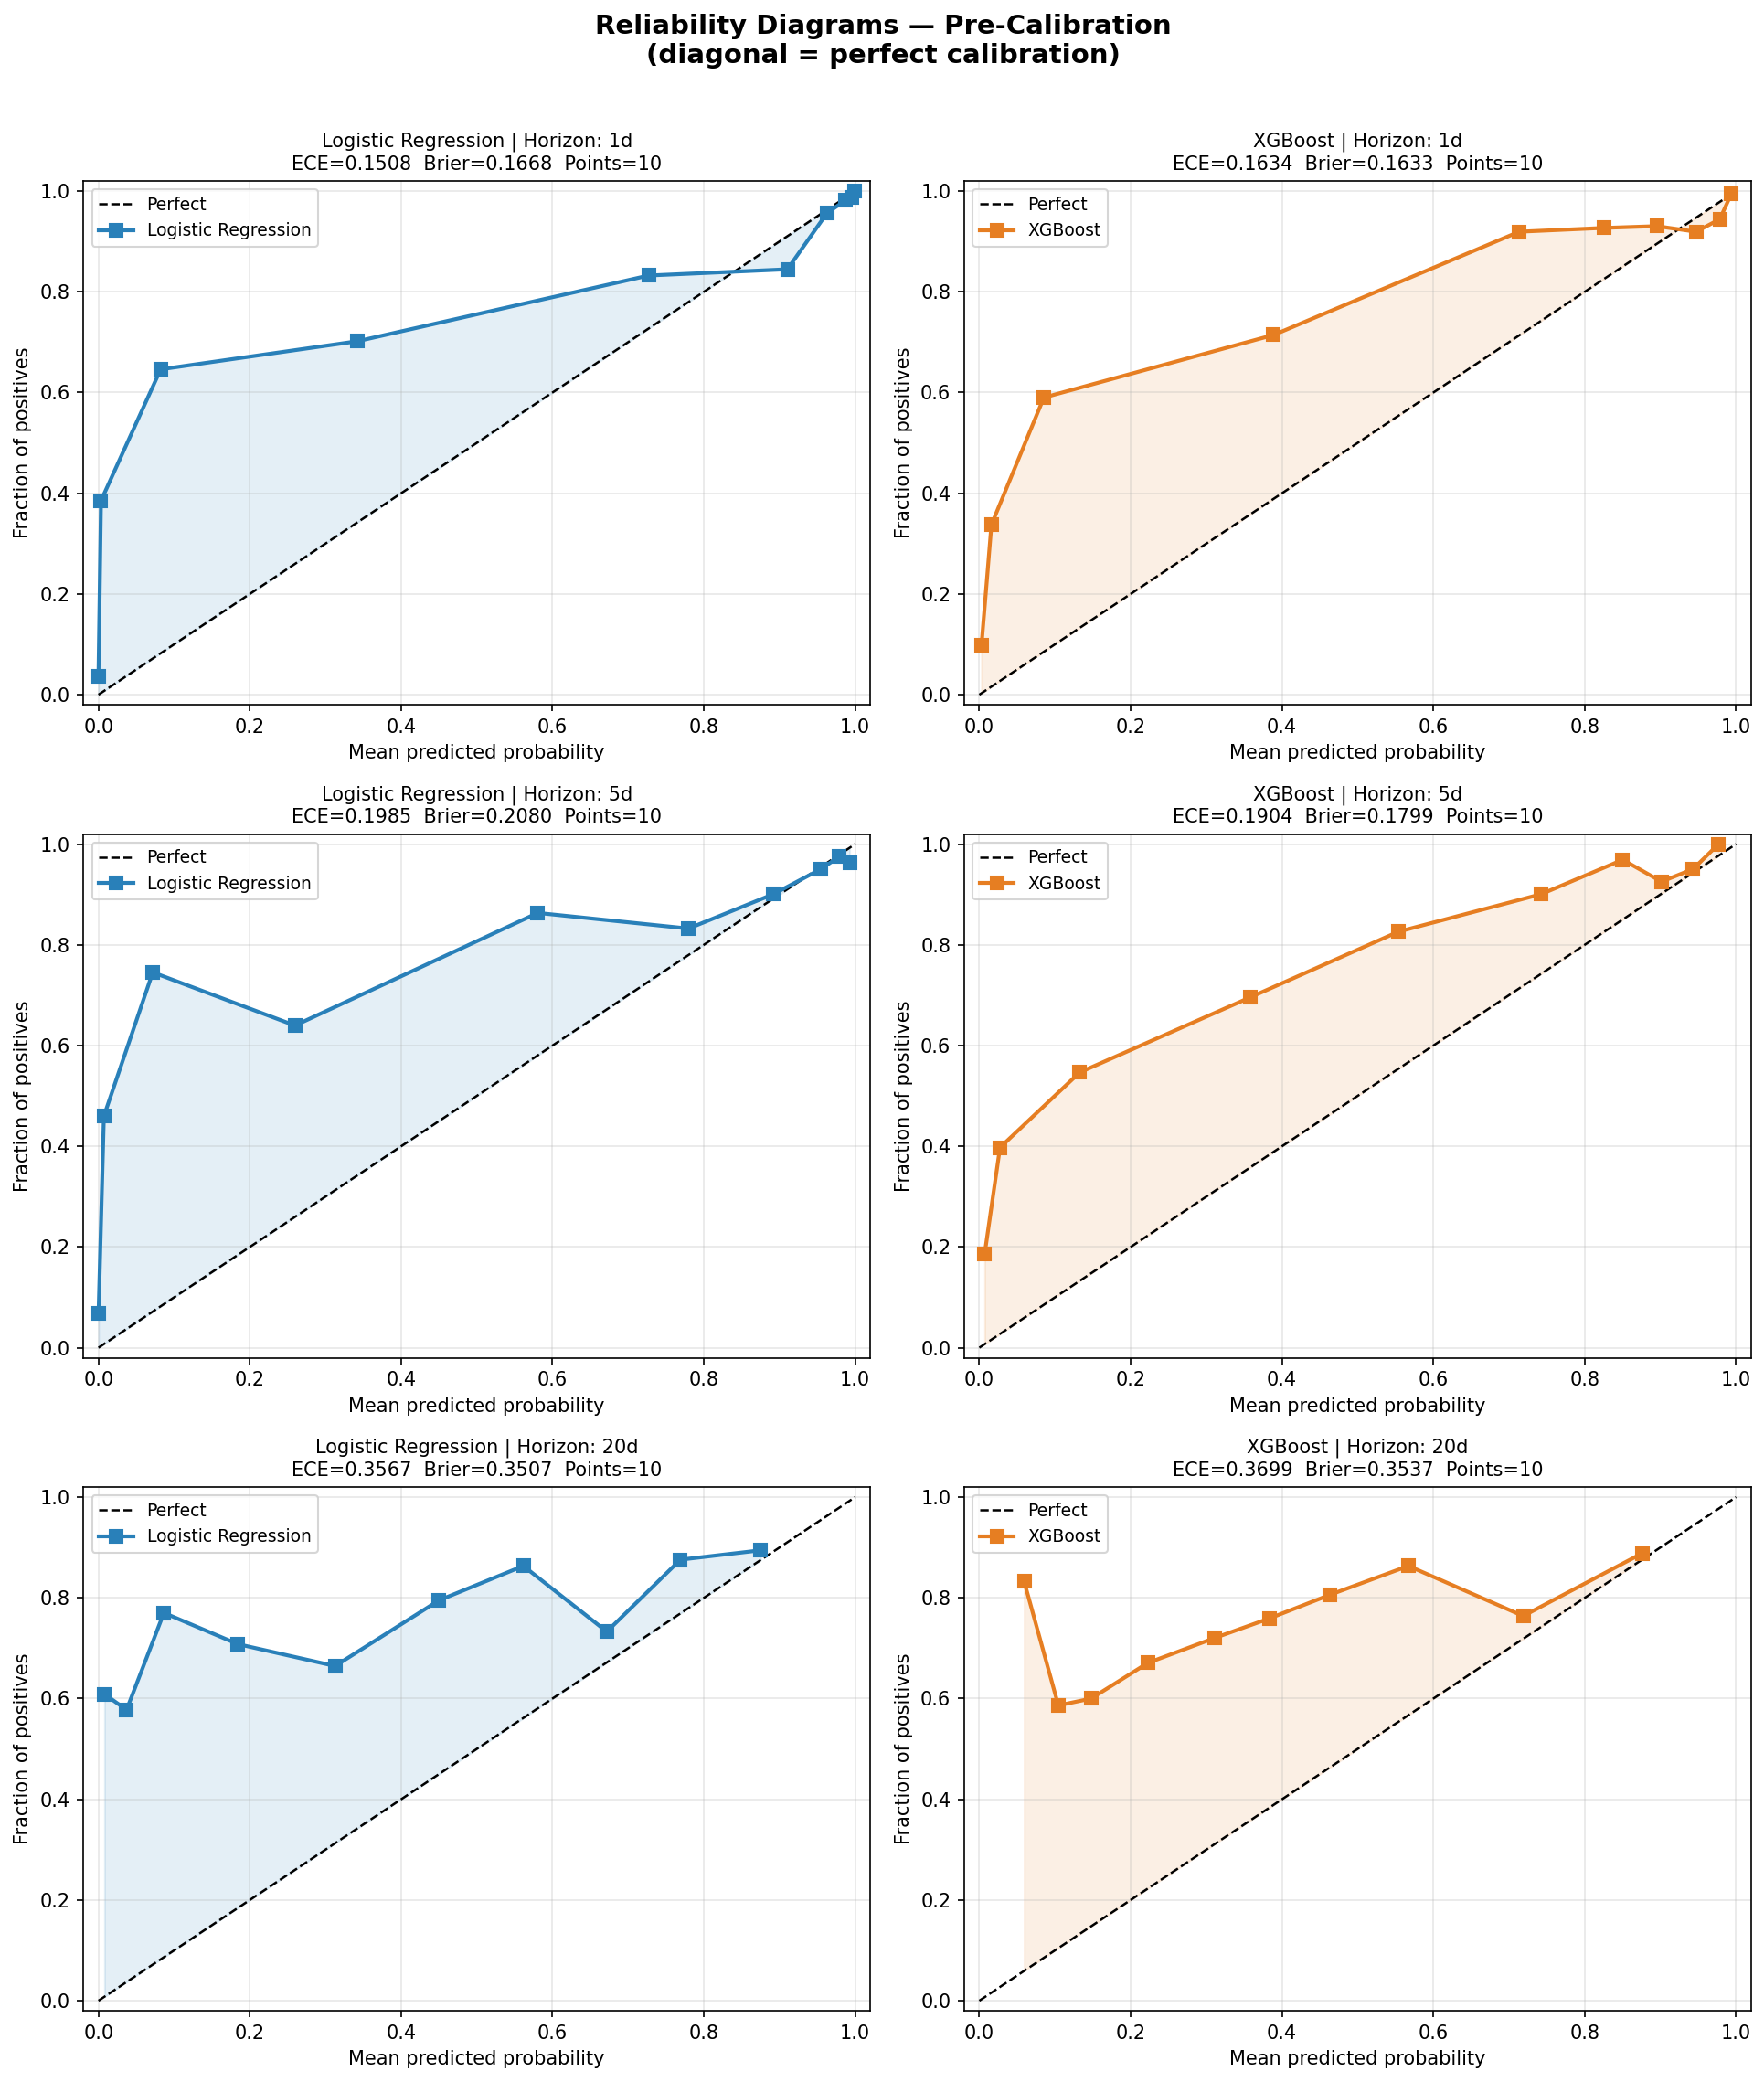
\includegraphics[width=0.92\linewidth]{../../reports/figures/calibration/reliability_pre_calibration.png}
\caption{Reliability diagrams before calibration for Logistic Regression (left)
and XGBoost (right) at horizons 1d, 5d, and 20d.
Dashed diagonal represents perfect calibration.
ECE and Brier Score are annotated per subplot.}
\label{fig:reliability-pre}
\end{figure}

% =====================================================================
\section{Results: Post-Calibration}
% =====================================================================

\subsection{Post-Calibration Metrics}

Table~\ref{tab:post-calib} reports the ECE after applying Platt Scaling and
Isotonic Regression to each model--horizon combination.

\begin{table}[H]
\centering
\caption{Post-calibration ECE on the test set.
``Platt'' = sigmoid calibration; ``Iso'' = Isotonic Regression.
$\Delta\text{ECE} = \text{ECE}_\text{raw} - \text{ECE}_\text{calibrated}$;
positive values indicate improvement.
Values to 3 significant figures.}
\label{tab:post-calib}
\begin{tabular}{llccccc}
\toprule
Horizon & Model & ECE (raw) & ECE (Platt) & $\Delta_\text{Platt}$ & ECE (Iso) & $\Delta_\text{Iso}$ \\
\midrule
\multirow{2}{*}{1 day}
  & Logistic & 0.151 & 0.163 & $-$0.012 & 0.159 & $-$0.008 \\
  & XGBoost  & 0.163 & 0.155 & $+$0.008 & 0.174 & $-$0.011 \\
\midrule
\multirow{2}{*}{5 days}
  & Logistic & 0.199 & 0.232 & $-$0.033 & 0.227 & $-$0.028 \\
  & XGBoost  & 0.190 & 0.150 & $+$0.041 & 0.215 & $-$0.025 \\
\midrule
\multirow{2}{*}{20 days}
  & Logistic & 0.357 & 0.381 & $-$0.024 & 0.443 & $-$0.086 \\
  & XGBoost  & 0.370 & 0.187 & $+$0.183 & 0.281 & $+$0.089 \\
\bottomrule
\end{tabular}
\end{table}

\subsection{Reliability Diagrams (Post-Calibration)}

Figure~\ref{fig:reliability-post} shows the reliability diagrams after calibration
for all four calibrated variants per horizon.
Effective calibration is evident when the plotted curve aligns more closely with
the perfect-calibration diagonal compared to Figure~\ref{fig:reliability-pre}.

\begin{figure}[H]
\centering
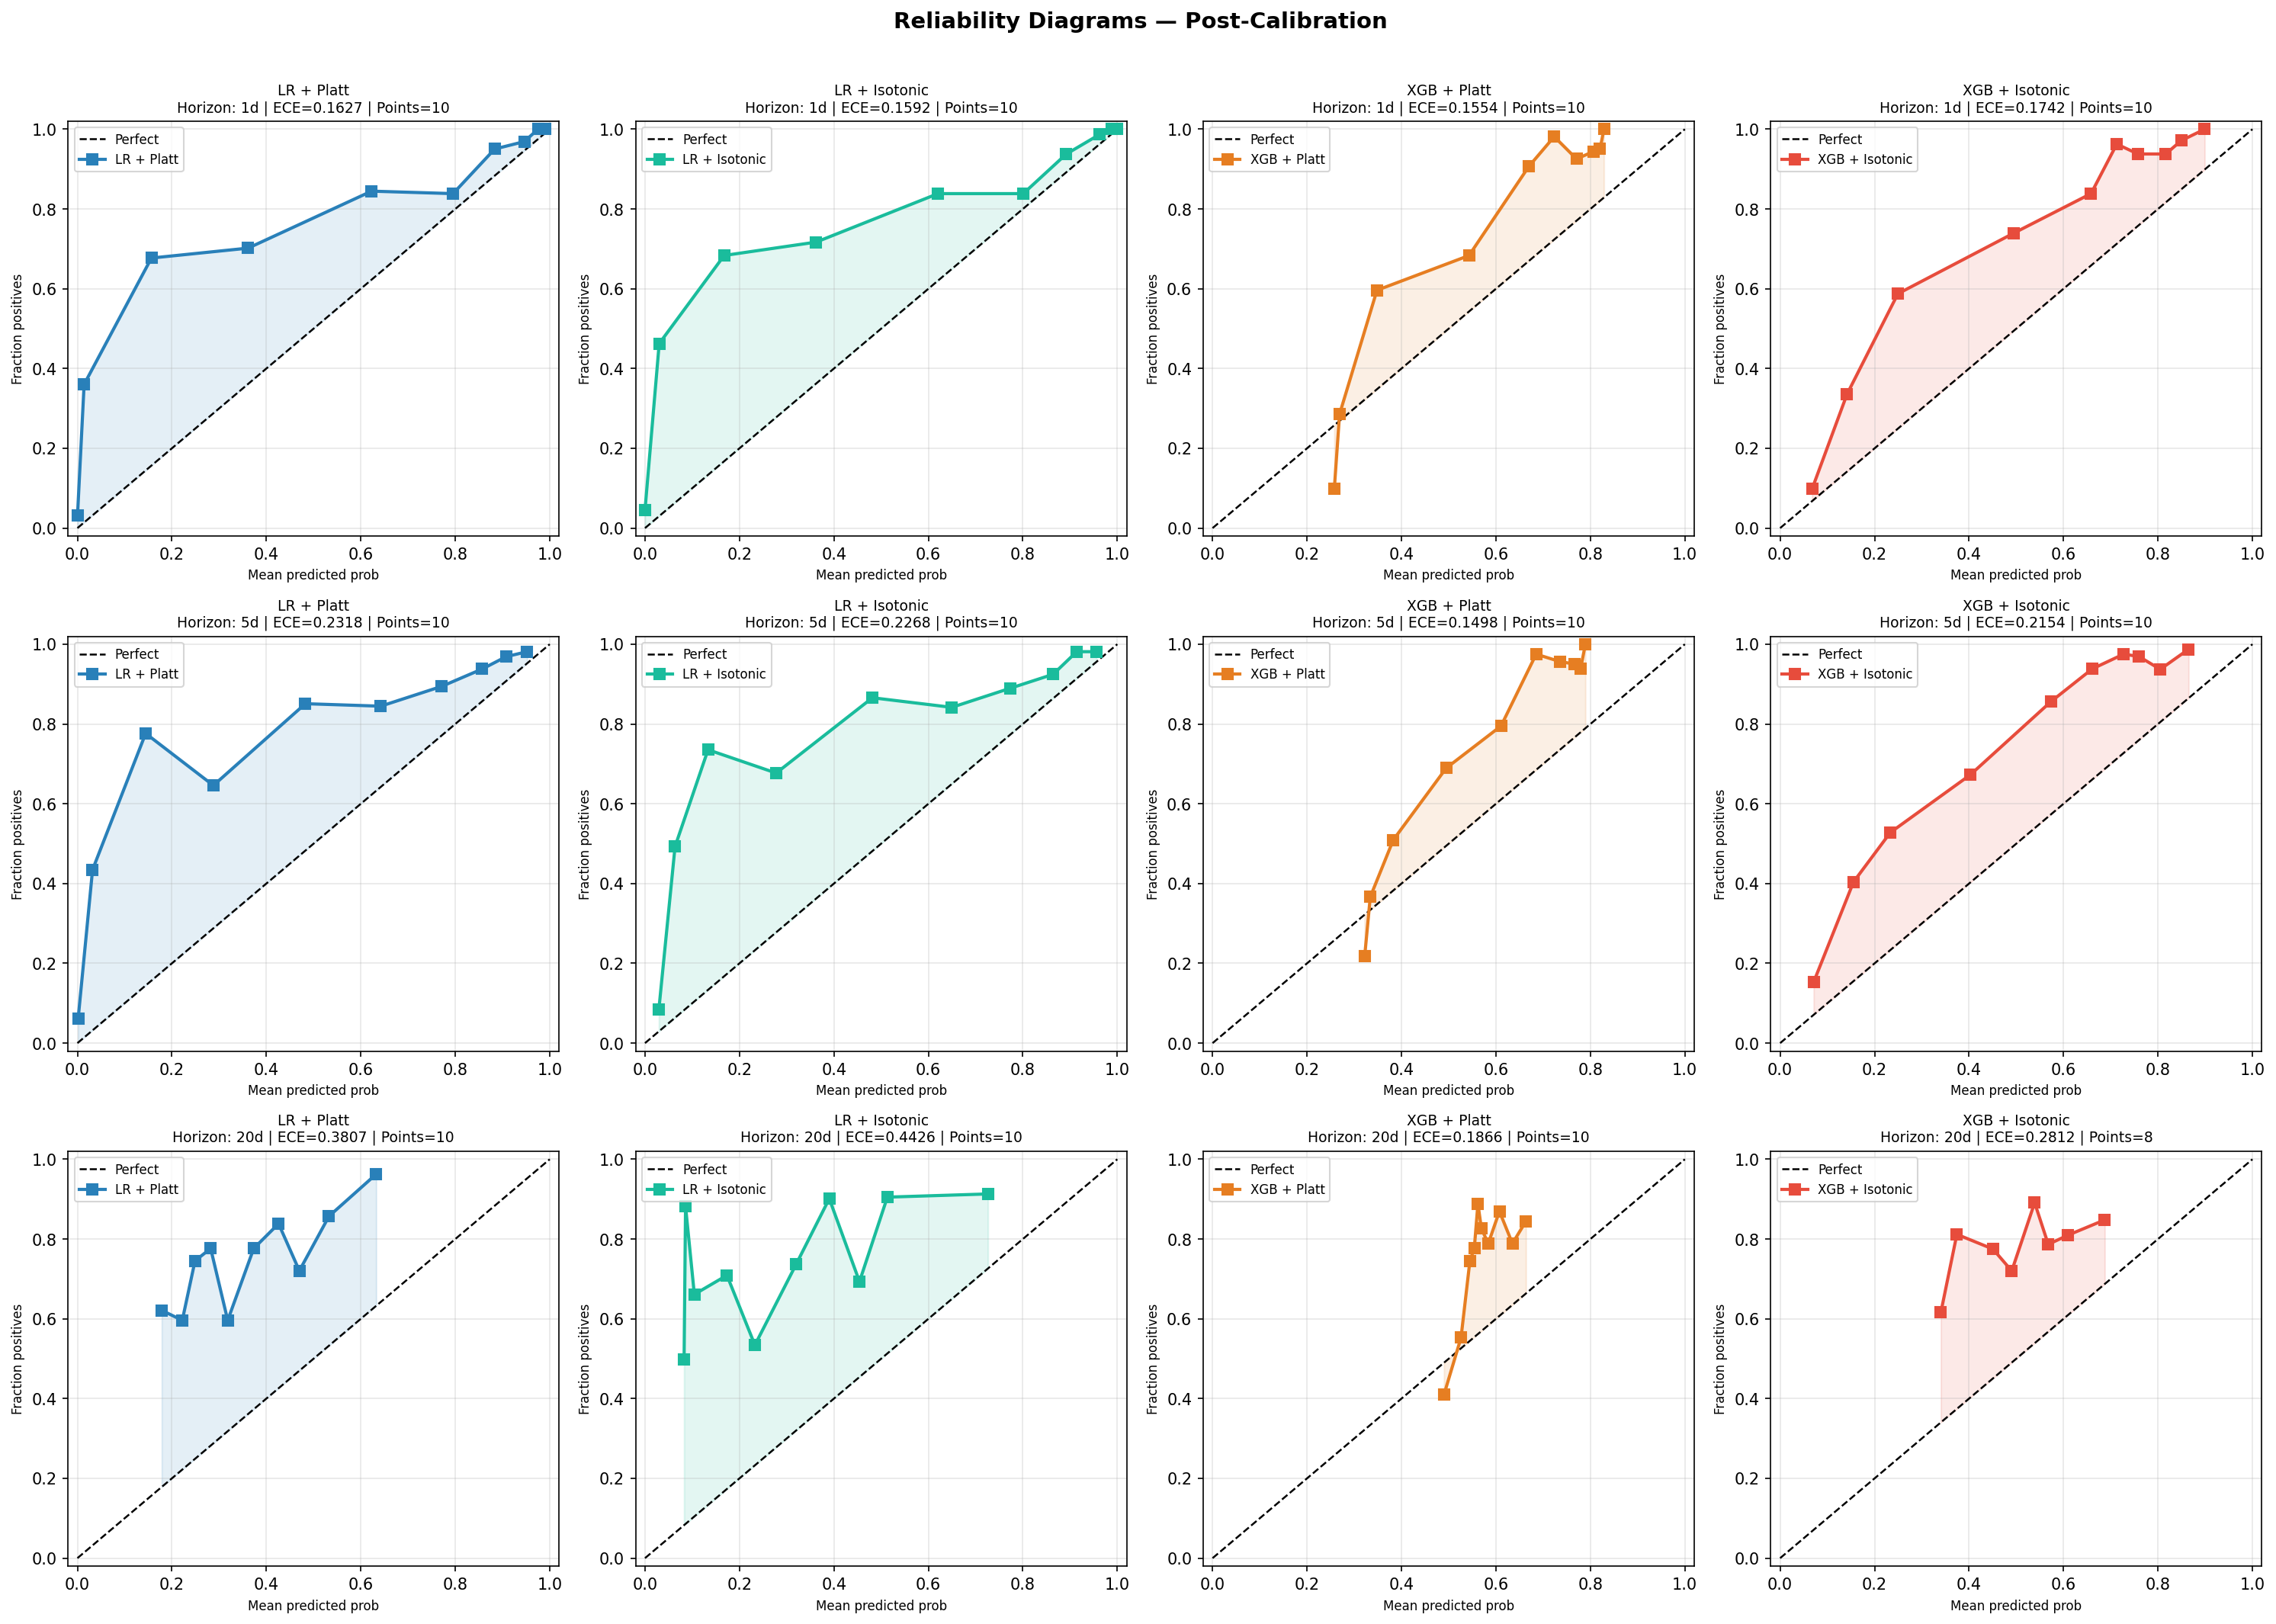
\includegraphics[width=0.92\linewidth]{../../reports/figures/calibration/reliability_post_calibration.png}
\caption{Reliability diagrams after calibration. Four variants per row:
LR+Platt, LR+Isotonic, XGB+Platt, XGB+Isotonic.
Rows correspond to horizons 1d (top), 5d (middle), 20d (bottom).}
\label{fig:reliability-post}
\end{figure}

% =====================================================================
\subsection{Hypothesis Evaluation}
% =====================================================================

\subsubsection{H1 --- XGBoost is Less Calibrated than Logistic Regression}

\textbf{Verdict: Partially supported.}

Examining Table~\ref{tab:pre-calib}, the ECE values per horizon are:
\begin{itemize}[leftmargin=1.5em,itemsep=2pt,topsep=4pt]
  \item \textit{1 day}: LR ECE = 0.151 $<$ XGB ECE = 0.163. \textbf{H1 supported.}
  \item \textit{5 days}: LR ECE = 0.199 $>$ XGB ECE = 0.190. \textbf{H1 violated.}
  \item \textit{20 days}: LR ECE = 0.357 $<$ XGB ECE = 0.370. \textbf{H1 supported.}
\end{itemize}

H1 holds at two out of three horizons.
The 5-day anomaly is noteworthy: at this horizon, XGBoost achieves lower ECE than
Logistic Regression.
This may reflect that, at intermediate forecast horizons, XGBoost's non-linear feature
interactions capture regime transitions more accurately, and the resulting
probability scores happen to align better with frequencies, possibly because
the model is less extreme in its assignments when uncertainty is higher.
By contrast, LR assigns moderate linear confidence even when the signal quality
is genuinely intermediate, which can inflate ECE.

It is important to note that ECE differences here are modest in absolute terms
(at most 0.013 at 1 day) and no formal significance test (e.g., a bootstrap confidence
interval on ECE) was applied.
Thus, the direction of the difference cannot be ascribed with statistical certainty.
A more rigorous test would compute bootstrap confidence intervals for each ECE estimate
and verify non-overlap.

\subsubsection{H2 --- Calibration Error Increases Monotonically with Horizon}

\textbf{Verdict: Fully supported for both models.}

The ECE values increase monotonically with horizon for both LR and XGB:
\begin{itemize}[leftmargin=1.5em,itemsep=2pt,topsep=4pt]
  \item LR: $0.151 \to 0.199 \to 0.357$ (1d $\to$ 5d $\to$ 20d). \checkmark
  \item XGB: $0.163 \to 0.190 \to 0.370$ (1d $\to$ 5d $\to$ 20d). \checkmark
\end{itemize}

This result is consistent with the informational decay hypothesis: as the prediction
horizon lengthens, the predictive signal in today's features degrades because market
regimes evolve, macro conditions shift, and the autocorrelation structure of the
regime label weakens.
The jump from 5 days to 20 days is substantially larger than from 1 day to 5 days,
suggesting a non-linear deterioration at longer horizons.
The AUC values in Table~\ref{tab:baseline-auc} corroborate this finding:
the 20-day AUC ($\approx 0.61$--$0.64$) is barely above chance.

H2 is the most robustly confirmed hypothesis.
The monotone trend holds without exception and with a sizeable magnitude at the
20-day horizon, making it unlikely to be attributable to noise.

\subsubsection{H3 --- Post-Calibration ECE Reduction is Greater for XGBoost}

\textbf{Verdict: Supported (with one minor exception under Isotonic at 1 day).}

Using Table~\ref{tab:post-calib}, the post-calibration reduction is
$\Delta\text{ECE}=\text{ECE}_{\text{raw}}-\text{ECE}_{\text{cal}}$.
For Platt Scaling, XGBoost improves at all horizons and by more than Logistic
Regression in each case:
$(+0.008, +0.041, +0.183)$ vs. LR $(-0.012, -0.033, -0.024)$
for 1d, 5d, and 20d respectively.

For Isotonic Regression, XGBoost also shows larger reduction than LR at 5d and 20d
($-0.025 > -0.028$ and $+0.089 > -0.086$), while at 1d both models worsen and
XGBoost is slightly worse than LR ($-0.011$ vs. $-0.008$).

Considering the best calibration choice per model-horizon pair,
XGBoost's reductions are positive at all horizons
($+0.008$, $+0.041$, $+0.183$), whereas LR's best available reductions remain
non-positive ($-0.008$, $-0.028$, $-0.024$).
Therefore, the central claim of H3 is empirically confirmed: XGBoost benefits
substantially more from post-hoc calibration than Logistic Regression,
with the strongest effect at 20 days.

% =====================================================================
\section{Discussion}
% =====================================================================

\subsection{Why Calibration Matters in Regime Prediction}

The analysis confirms that calibration quality deteriorates substantially at the
20-day horizon for both models, with ECE values exceeding 0.35.
In practical terms, this means predictions in the highest-confidence bin are off
by more than 35 percentage points on average.
A portfolio manager relying on these raw probabilities to size positions at a
20-day rebalancing frequency would systematically over-allocate to high-confidence
signals.
Post-hoc calibration is therefore not merely a statistical nicety but a prerequisite
for sound decision-making at longer horizons.

\subsection{Limitations}

Several limitations warrant acknowledgement.
First, the ECE metric is sensitive to the number of bins $B$: choosing $B=10$
is conventional but can produce noisy estimates when bins are sparsely populated,
as is likely at the extremes of the probability range for the 20-day horizon.
Second, the 80/20 chronological split means the test set (2019--2026) spans
the COVID-19 crash and the post-pandemic recovery, a period of atypical regime
dynamics that may not represent the long-run distribution.
Third, no formal statistical test was applied to the ECE differences reported
in H1; bootstrap confidence intervals would be necessary for definitive claims
about relative calibration quality.

\subsection{Comparison of Calibration Methods}

Platt Scaling is preferred when the miscalibration is expected to be monotone
and the calibration dataset is small (the parametric form regularises the fit).
Isotonic Regression is preferred when the reliability curve has a non-trivial
shape and sufficient data are available to estimate a piecewise function without
overfitting.
Given the 1,610-observation test set, Isotonic Regression has 160 observations
per bin on average (for $B=10$), which is generally adequate; however, the tails
of the distribution may be sparsely populated.
In practice, both methods should be compared empirically (as done here), and the
choice made on the basis of out-of-sample ECE.

% =====================================================================
\section{Conclusion}
% =====================================================================

This study evaluated the calibration of Logistic Regression and XGBoost classifiers
for bull/bear equity-regime prediction across three forecast horizons (1d, 5d, 20d).
The key findings are:

\begin{itemize}[leftmargin=1.5em,itemsep=2pt,topsep=4pt]
  \item \textbf{H1} is \emph{partially} supported: XGBoost is less calibrated than
    Logistic Regression at 1-day and 20-day horizons, but slightly better calibrated
    at 5 days.
    The differences are small in absolute terms and should be interpreted cautiously
    without a formal significance test.
  \item \textbf{H2} is \emph{fully} supported: calibration error increases
    monotonically with horizon for both models.
    The degradation is especially severe at 20 days, where ECE exceeds 0.35,
    making raw probabilities unsuitable for direct use in financial decision-making.
  \item \textbf{H3} is supported: post-hoc calibration yields larger ECE reduction
    for XGBoost than for Logistic Regression overall.
    Under Platt Scaling, XGBoost improves at all horizons while LR worsens.
    Under Isotonic Regression, XGBoost still outperforms LR at 5 and 20 days,
    with only a minor 1-day exception where both models deteriorate.
\end{itemize}

The results highlight that discriminative accuracy (AUC) and calibration quality
are complementary, not equivalent, criteria.
Both models achieve high AUC at short horizons while remaining substantially
miscalibrated.
Post-hoc calibration via Platt Scaling or Isotonic Regression should be applied
as a standard step in any probabilistic regime-prediction pipeline, particularly
at longer forecast horizons.

% =====================================================================
\section*{References}
% =====================================================================

\small
\begin{itemize}[leftmargin=1.5em,itemsep=1pt,topsep=4pt]
  \item Guo, C., Pleiss, G., Sun, Y., and Weinberger, K.~Q. (2017). On calibration
    of modern neural networks. \textit{Proceedings of the 34th International
    Conference on Machine Learning (ICML)}, pp.\ 1321--1330.
  \item Niculescu-Mizil, A. and Caruana, R. (2005). Predicting good probabilities
    with supervised learning. \textit{Proceedings of the 22nd International
    Conference on Machine Learning (ICML)}, pp.\ 625--632.
  \item Platt, J.~C. (1999). Probabilistic outputs for support vector machines and
    comparisons to regularized likelihood methods.
    \textit{Advances in Large Margin Classifiers}, pp.\ 61--74.
  \item Widmann, D., Lindsten, F., and Zachariah, D. (2019). Calibration tests in
    multi-class classification: A unifying framework.
    \textit{Advances in Neural Information Processing Systems (NeurIPS)}, 32.
  \item Zadrozny, B. and Elkan, C. (2002). Transforming classifier scores into
    accurate multiclass probability estimates. \textit{Proceedings of the 8th ACM
    SIGKDD International Conference on Knowledge Discovery and Data Mining},
    pp.\ 694--699.
\end{itemize}

\section*{AI Disclosure}
AI tools (Perplexity AI) were used to support report structuring, LaTeX
formatting, and proofreading.
All methodology choices, numerical results, and hypothesis evaluations were
derived directly from the notebook outputs and reviewed by the author.

\end{document}